% -*-latex-*-
%
%  The contents of this file are subject to the University of Utah Public
%  License (the "License"); you may not use this file except in compliance
%  with the License.
%
%  Software distributed under the License is distributed on an "AS IS"
%  basis, WITHOUT WARRANTY OF ANY KIND, either express or implied. See the
%  License for the specific language governing rights and limitations under
%  the License.
%
%  The Original Source Code is SCIRun, released March 12, 2001.
%
%  The Original Source Code was developed by the University of Utah.
%  Portions created by UNIVERSITY are Copyright (C) 2001, 1994
%  University of Utah. All Rights Reserved.
%

% running.tex
%
% This is the `Running SCIRun' main section.

%begin{latexonly}
  \newcommand{\srwindow}%
  {\centerline{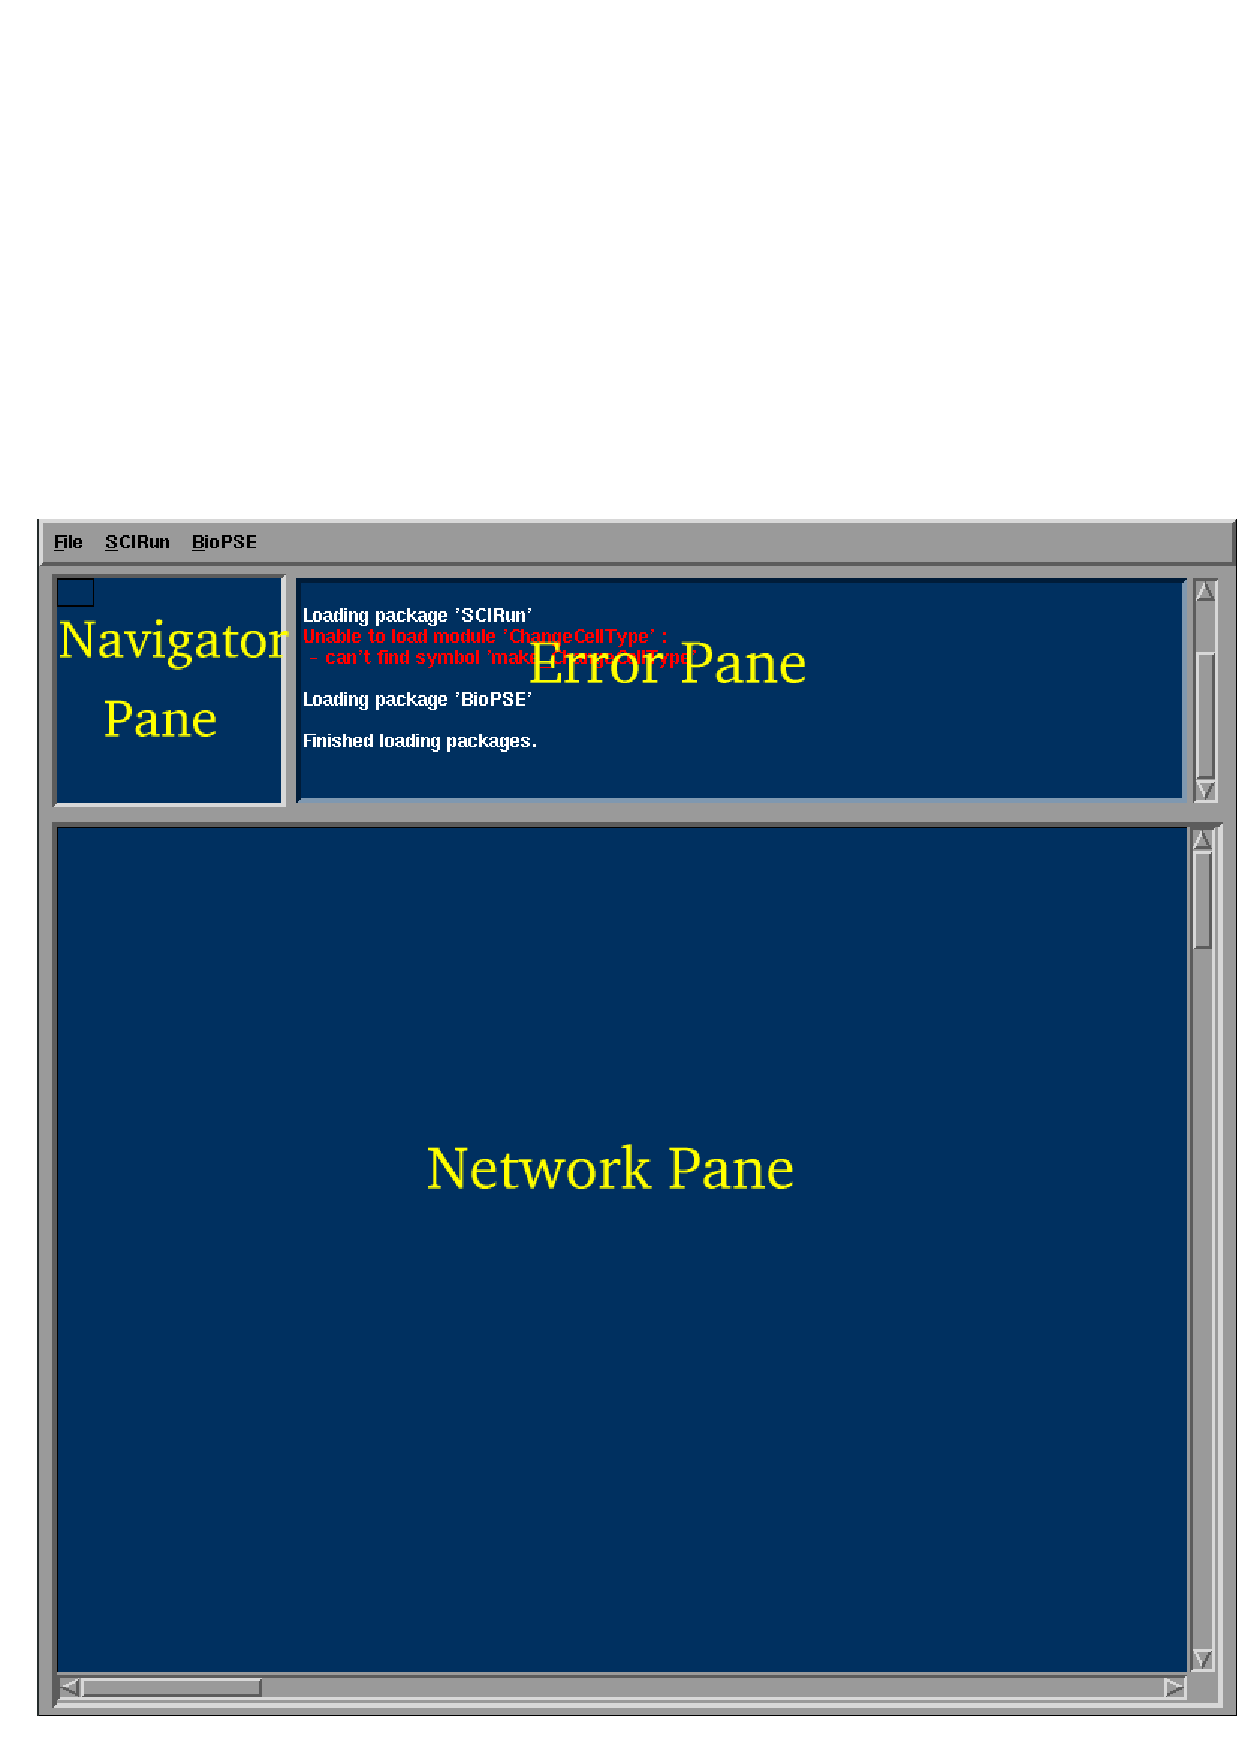
\epsfig{file=Figures/srwindow-1.eps.gz, width=6in,
        bbllx=0, bblly=0, bburx=400, bbury=410}}}
%end{latexonly}
\begin{htmlonly}
  \newcommand{\srwindow}{%
  \htmladdimg[align=top,alt="SCIRun Window"]
  {../Figures/srwindow-1.gif}}
\end{htmlonly}


\section{Starting \sr{}}
\label{sec:startingup}

\subsection{The \command{scirun} Command}
\label{sec:sciruncmd}

Start \sr{} by typing \keyboard{scirun} in a terminal (\eg \command{xterm})
window.  \note{Don't start \sr{} in the background, \ie don't type
\keyboard{scirun \&}}.

The \command{scirun} command is located in the
\directory{src} directory of the \directory{\sr} install directory.  The
person who installed \sr{} can locate this command for you.


\begin{figure}[htb]
  \begin{makeimage}
  \end{makeimage}
  \srwindow
  \caption{\label{fig:srwindow} \sr{} Main Window}
\end{figure}


Typing \keyboard{scirun} with no arguments starts up \sr{} with a blank \sr{}
window as shown in Figure~\ref{fig:srwindow}.  The main features of this
window are discussed in \secref{Anatomy of the Main
  Window}{sec:windowanatomy}.

The \command{scirun} command may take 1 argument
which is the name of a \sr{} \dfn{network} \index{network} file (these
files have a \filename{.net} extension).  These files hold previously
defined \sr{} networks.  \sr{} will load the specified network.  Network
files will be discussed in a later section.

\sr{} may encounter errors during start up.  These will be displayed in
\sr{}'s error frame (see Figure~\ref{fig:srwindow}).  These errors
should be \htmladdnormallink{reported}{\bugsurl} to the \sr{} development
team.  \latexonly{See \secref{Reporting Bugs}{sec:bugs} for information on
  reporting bugs.}

\subsection{Anatomy of the Main Window}
\label{sec:windowanatomy}

The \sr{} main window consists of 4 main components (see
Figure~\ref{fig:srwindow}): 

\begin{description}
\item[Menu Bar] The menu bar is used to load networks, save networks, quit
  \sr{}, create network modules, and perform other tasks.  The menu bar
  consists of the following menu items:

  \begin{description}
  \item[\menu{File}] The \menu{File} menu contains the following items:
    \begin{description}
    \item[Save] Saves the current network to a file.
    \item[Load] Loads a network from a file.
    \item[New] This sub-menu contains items of interest to developers only.
    \item[Add Info] Use this item to add network specific notes to
      the current network.  Notes should be used to document the purpose of
      the network.
    \item[Quit] Quits \sr{}.
    \end{description}
  \end{description}
  
  \begin{description}
  \item[\menu{SCIRun}] The \menu{SCIRun} menu is used to create modules
    (from the \sr{} package) for use in the net edit frame.  This menu is
    composed of sub-menus. Each sub-menu corresponds to a \dfn{category}
    \index{category} within the \sr{} package.  A category is a group of
    related modules.  Each menu item in a category sub-menu creates a
    specific module and places it in the netedit frame.  The netedit frame
    pop-up menu (activated by clicking the right most mouse button when the
    mouse pointer is in the netedit frame) also provides access to the
    \menu{\sr{}} and \menu{\pse{}} (and possibly other) package menus.  An
    overview of the contents of the \sr{} package is given in \secref{The
      \pse{} Package}{sec:biopsepackage}.
  \end{description}

  \begin{description}
  \item[\menu{BioPSE}] The \menu{BioPSE} menu is used to create modules
    (from the \pse package) for use in the netedit frame.  It consists
    of category sub-menus and module menu items.   An overview of the
    contents of the \sr{} package is given in \secref{The SCIRun
      Package}{sec:srpackage}.
  \end{description}

  \begin{description}
  \item [\textit{Other Package Menus}] There may be other package
    menus if other packages have been installed.  They too will consist
    of category sub-menus and module menu items.
  \end{description}
  
\item[Global View Frame] The Global View Frame is located in the upper left
  corner of the main window (see Figure~\ref{fig:srwindow}). It is used to
  navigate complex networks.  The use of the Globla View Frame will be
  described in \secref{Navigating a Network}{sec:navnetwork}.
  
\item[Error Frame] Errors during program startup are displayed in the Error
  Frame.  It is located in the upper right corner of the main window(see
  Figure~\ref{fig:srwindow}).  Errors on startup may mean that \sr{} has
  been installed incorrectly or has been installed from a buggy
  distribution.  Please \hyperref{report}{(see Section~}{)}{sec:bugs} these
  errors.
  
\item[NetEdit Frame] The NetEdit Frame occupies the bottom of the main
  window(see Figure~\ref{fig:srwindow}).  It is used to build and execute
  networks.  \secref{Building Networks}{sec:workwithnets} discusses the use
  of this frame.

\end{description}

\subsection{The Terminal Window}
\label{sec:termwinapp}

After starting, \sr{} will also run a shell-like application in the
terminal window called the \dfn{\sr{} shell}.  The \sr{} shell displays the
prompt \screen{scirun\ra}.  This program is actually a modified \dfna{Tool
  Command Language}{TCL} shell program and it is possible to type in
\acronym{TCL}'ish \sr{} commands at the prompt. The use of this program
will be described in \hyperref{a later section}{Section~}{}{sec:termapp}.


\subsection{Environment Variables}
\label{sec:environ} 
\index{Environment Variables}

There are several environment variables that \sr{} uses to make it easier
to use.  These are all optional, but paying attention to them can make it
easier to find files during a \sr{} session and to improve performance via
remote connections.

\begin{description}
  \item[{\envvar{SCIRUN\_DATA}}\mbox{}: ]\mbox{}
        \index{SCIRUN\_DATA}
        \label{sec:scirundata}
        The environment variable \envvar{SCIRUN\_DATA} specifies the
        default directory of \sr{} data files.  \sr{} will first look
        in this directory to find data and network files.  It affects
        the behavior of file browsing dialogs --- they will prompt for
        a file within the \envvar{SCIRUN\_DATA} directory (of course
        you may have the dialog look elsewhere).  This can be very
        handy when using shared datasets, like the one shipped with
        the software.  Many of the demonstration nets with the
        software also assume that \envvar{SCIRUN\_DATA} points to the
        location of these datasets.

  \item[\envvar{SCIRUN\_DATASET}\mbox{}: ]\mbox{}
        \label{sec:scirundataset} 
        This variable refines the search for data files within the
        directory pointed at by \envvar{SCIRUN\_DATA}.  By setting
        these two variables, one can easily select different data sets
        for the same network.  See the network files distributed with
        the software, for example \filename{forward-fem.net}, so
        examples of how to use these variables.  Some of the
        demonstration nets do require setting \envvar{SCIRUN\_DATASET}
        so see the documentation on those.

      \item[\envvar{DISPLAY}: ]\mbox{}
        
        If \sr is executed remotely then the value of the
        \envvar{DISPLAY} variable (as set on the remote machine) must
        be set correctly and the remote machine must be allowed to
        talk to the local X11 server.
        
        For telnet-like (unencrypted) connections to a remote machine
        you may set \envvar{DISPLAY} as follows:

\begin{verbatim}
  export DISPLAY=local-ip-addres:0.0
\end{verbatim}
        
        for an sh-style shell. And like this:

\begin{verbatim}
setenv DISPLAY local-ip-addres:0.0
\end{verbatim}

        for a csh-style shell.

        When connecting to a remote machine using ssh, \envvar{DISPLAY} is
        normally set automatically (depending on how ssh has been
        configured).  This results in poor display performance however
        because of encryption activity on the connection.  To increase
        performance you may override the value of \envvar{DISPLAY} provided
        by ssh.  Simply set \envvar{DISPLAY} as
        shown above.  Note that this technique defeats the encryption
        protection on the X11 connection.

        You will need to grant the remote machine permission to display on
        your local machine if you are using a telnet-like connection or if
        you are overriding the value of \envvar{DISPLAY} provided by ssh.
        Use the \command{xhost} command on the local machine to do
        this:

\begin{verbatim}
xhost +remote-machine-name
\end{verbatim}

  \item[\envvar{SCI\_ON\_THE\_FLY\_LIBS\_DIR}\mbox{}: ]\mbox{}
    
    \envvar{SCI\_ON\_THE\_FLY\_LIBS\_DIR} specifies the location of
    dynamically generated code.  See \secref{Dynamic
      Compilation}{sec:dyncomp} for details on the meaning and use of
    this variable.

    
\end{description}

\subsection{\sr{}'s Initialization File---\filename{.scirunrc}}
\label{sec:scirunrc}

One of the first thing \sr{} does when it starts up is to look for and
load the content of the file \filename{.scirunrc}.  \sr{} searches for
\filename{.scirunrc} in this order:

\begin{enumerate}
\item The current working directory.
\item The root of \sr;'s build directory.
\item Your home directory.
\item The root of \sr;'s source code directory.
\end{enumerate}

This file may contain assignment of values to variables and variable
substitution:

\begin{verbatim}
HOME=/home/sci/me
SCIRUN_ON_THE_FLY_LIBS_DIR=$(HOME)/on-the-fly-libs
\end{verbatim}

The expansion of environment variables is not supported.  Only
variables declared earlier in the file may be expanded.

The following variables are understood by \sr{} and may be set in
\filename{.scirunrc}: \envvar{SCI\_ON\_THE\_FLY\_LIBS\_DIR},
\envvar{LOAD\_PACKAGE}, \envvar{PACKAGE\_SRC\_PATH},
\envvar{PACKAGE\_LIB\_PATH}.

\secref{Dynamic Compilation}{sec:dyncomp} explains the meaning and use
of \envvar{SCI\_ON\_THE\_FLY\_LIBS\_DIR}.

Here are the meanings of the other variables:

\begin{description}
  \item[\envvar{LOAD\_PACKAGE}\mbox{}: ]\mbox{} 
    
    A comma seperated list of package names that \sr{} will load.
    
    This overrides the packages specified at configure time.  Note
    that this will not cause packages not specifed at configure time
    to magically compile and load though!  The package must already be
    compiled.  Whitespace is not tolerated after commas.
    
    Its value defaults to the list of packages given to the
    \option{\-\-enable-package} option at configure time.
    
  \item[\envvar{PACKAGE\_SRC\_PATH}\mbox{}: ]\mbox{} 
    
    A colon separated list of paths to root(s) of package source
    trees.  The path \directory{\ptext{build\_dir}/Packages} is implicitly part of
    this list.  Note that \ptext{build\_dir} is the directory in which
    the \command{configure} and \command{make} commands were run.
   
    \sr{} searches this path list to find XML description files and
    user interface code corresponding to the list of packages
    specified in \envvar{LOAD\_PACKAGE}.
    
    It's value defaults to \directory{\ptext{build\_dir}/Packages}.

  \item[\envvar{PACKAGE\_LIB\_PATH}\mbox{}: ]\mbox{} 
    
    \envvar{PACKAGE\_LIB\_PATH} is a colon separated list of paths to
    package libraries.
    
    \sr{} searches this path list to find package libraries
    which correspond to the list of packages specified in
    \envvar{LOAD\_PACKAGE}.
    
    It's default value is \directory{\ptext{build\_dir}/lib}.

\end{description}

\subsection{Dynamic Compilation}
\label{sec:dyncomp}

Before executing \sr{} you should be aware of a feature called
\dfn{Dynamic Compilation}.

Dynamic compilition is a technique used by \sr{} that discovers and
generates code for the data types and algorithms used by modules in
your networks.  This is done at runtime and is done once for each new
data type and algorithm encountered.  This technique provides a number
of benefits not discussed here.  See
\htmladdnormallinkfoot{\etitle{Dynamic
    Compilation}}{http://www.sci.utah.edu/publications/mcole01/dyn.pdf}
  for details.

By default, code generated by dynamic compilation is stored in the
directory \directory{\ptext{build\_dir}/on-the-fly-libs} (where
\ptext{build\_dir} is the directory in which \sr{} was built).  The
location of dynamically generated code can be changed (and doing so
provides a number of benefits---see below) by setting the value of the
environment variable \envar{SCI\_ON\_THE\_FLY\_LIBS\_DIR} to the
desired directory, for example:

\begin{verbatim}
SCIRUN_ON_THE_FLY_LIBS_DIR=$Home/on-the-fly-libs
export SCIRUN_ON_THE_FLY_LIBS_DIR
\end{verbatim}

for Bourne-like shells (sh, ksh, bash, etc.) or

\begin{verbatim}
setenv SCIRUN_ON_THE_FLY_LIBS_DIR $HOME/on-the-fly-libs
\end{verbatim}

for csh-like shells.

It can also be changed by setting the value of this variable in
your \filename{.scirunrc}
file. Your \filename{.scirunrc} file would contain, for example:

\begin{verbatim}
SCIRUN_ON_THE_FLY_LIBS_DIR=/home/me/on-the-fly-libs
\end{verbatim}

Your \filename{.scirunrc} file is read by \sr{} at startup.

Customizing the value of this variable for each \sr{} user has
the following benefits:

\begin{itemize}
\item It allows multiple users to run the same instance of \sr{} (at
the same time) without worrying about dynamic compilation conflicts.
For example, by specifying an \filename{on-the-fly-libs}
directory in their home directory, a user can run the same shared
\sr{} installed in \directory{/usr/local} that another user
is already running.

\item It allows a \directory{/usr/local} installation of \sr{}
to be secure by not requiring that
\directory{/usr/local/.../on-the-fly-libs} be writable by
all (which is considered a potential security risk).

\item It allows greater debugging and multiple build support by
allowing the user to change dynamically compiled code locations
between instances of \sr{}.

\end{itemize}

Dynamic compilition will cause a delay the first time a module is
executed.  The module will turn a different color while it is being
compiled.

\subsection{Quitting or Exiting \sr{}}
\label{sec:stopping}

Quit \sr{} by selecting the \menuitem{Quit} item from the \menu{File} menu

\warning{Don't press \keyboard{control-c} to exit \sr{}.  Doing this will
drop you into a debugger which is probably not what you want to do}.


%%% Local Variables: 
%%% mode: latex
%%% TeX-master: "usersguide"
%%% End: 
